\def\tutdate{19.01.2017}
\ifdefined\compileall \else
\ifdefined\compiletype
	\documentclass[handout]{beamer}
\else
	\documentclass{beamer}
	\def\compiletype{livebeamer}
\fi

\usepackage{templates/beamerthemekitwide}

\usepackage[utf8]{inputenc}
\usepackage[T1]{fontenc}
\usepackage[ngerman]{babel}
\usepackage{listings}
\usepackage{hyperref}
\usepackage{graphicx}

\usepackage{amsmath}
\usepackage{amsthm}
\usepackage{amssymb}
\usepackage{polynom}

\usepackage{ifthen}
\usepackage{adjustbox} % for \adjincludegraphics

\newcommand{\markBlue}[1]{\textcolor{kit-blue100}{#1}}
\newcommand{\markGreen}[1]{\textcolor{kit-green100}{#1}}

\newcommand{\pitem}{\pause\item}
\newcommand{\p}{\pause}

% -- MATH MACROS
\newcommand{\thistheoremname}{}
\newcommand{\G}{\mathbb{Z}}
\newcommand{\B}{\mathbb{B}}
\newcommand{\R}{\mathbb{R}}
\newcommand{\N}{\mathbb{N}}
\newcommand{\Q}{\mathbb{Q}}
\newcommand{\C}{\mathbb{C}}
\newcommand{\Z}{\mathbb{Z}}
\newcommand{\F}{\mathbb{F}}
\newcommand{\mi}{\mathrm{i}}
\renewcommand{\epsilon}{\varepsilon}


\newenvironment<>{taskblock}[1]{%
	\setbeamercolor{block title}{fg=kit-orange15,bg=kit-orange100}
	\setbeamercolor{block body}{fg=black,bg=kit-orange30}%
	\begin{block}#2{#1}}{\end{block}}

\setbeamertemplate{enumerate items}[default]

% Aussagenlogik Symbole
\newcommand{\W}{w}
\renewcommand{\F}{f}

% Kodierung
\newcommand{\frepr}{\textbf{repr}}
\newcommand{\fRepr}{\textbf{Repr}}
\newcommand{\fZkpl}{\textbf{Zkpl}}
\newcommand{\fbin}{\textbf{bin}}
\newcommand{\fdiv}{\textbf{ div }}
\newcommand{\fmod}{\textbf{ mod }}

\title[Grundbegriffe der Informatik]{Grundbegriffe der Informatik\\Tutorium 33}
\subtitle{}
\author{Lukas Bach, lukas.bach@student.kit.edu}
\date{\tutdate}

\institute{}

\titlelogo{lukasbach}

\titleimage{bg}
%\titleimage{bg-advent}


\ifthenelse{\equal{\compiletype}{livebeamer}}
	{
		\def\livebeamermode{1}
	}{}

\ifthenelse{\equal{\compiletype}{print}}
	{
		\def\printmode{1}
	}{}

\setbeamercovered{invisible}

%\usepackage[citestyle=authoryear,bibstyle=numeric,hyperref,backend=biber]{biblatex}
%\addbibresource{templates/example.bib}
%\bibhang1em

\begin{document}
	
\selectlanguage{ngerman}


%title page
\begin{frame}
	\titlepage
\end{frame}

%table of contents
\ifdefined\printmode
	\ifdefined\compileall \else
	\begin{frame}{Gliederung}
		\tableofcontents
	\end{frame}
\fi\fi

\fi

\section{Repräsentation von Graphen}
\begin{frame}{Repräsentation von Graphen}
	Wie stellen wir Graphen da?\\\ip
	\center{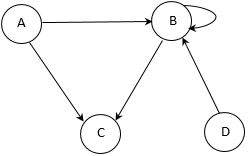
\includegraphics[scale=0.6]{images/Graph1.png}}\\
	Anschaulich ja, aber wie können wir Graphen z.B. mit Java realisieren?
\end{frame}

%Selber drauf kommen lassen
\begin{frame}{Objektorientierte Repräsentation von Graphen}
	Klassenmodell?\pause
	
	\begin{alltt}
		class Vertex \{ 					\\                                  
		\hspace{0.4cm} String name; //Genauer Inhalt interessiert uns nicht	\\                               
		\}   
		\vspace{0.3cm}        			\\               
		class Edge \{ 					\\ 
		\hspace{0.4cm}	Vertex start;    \\
		\hspace{0.4cm}	Vertex end;     \\
		\}  
		\vspace{0.3cm}                    \\               
		class Graph \{					\\
		\hspace{0.4cm}   Vertex[] vertices;\\
		\hspace{0.4cm}   Edge[] edges;	\\
		\}								\\
	\end{alltt}
\end{frame}

\begin{frame}{Objektorientierte Repräsentation von Graphen}
	\begin{itemize}
		\pitem[\textbf{+}] Intuitiv
		\pitem[\textbf{--}] Es lassen sich nur schwer Algorithmen hierfür entwerfen (z.B. gilt $(x,y) \in E$?)
	\end{itemize}
\end{frame}

\subsection{Adjazenzlisten}
\begin{frame}{Repräsentation mit Adjazenzlisten}
	Jeder Knoten speichert seine Nachbarn:
	\begin{alltt}
		class Vertex \{ 					\\                                  
		\hspace{0.4cm} String name; //Genauer Inhalt interessiert uns nicht	\\                               
		\hspace{0.4cm}   \textcolor{blue}{Vertex[] neighbours;} //Alle Nachbarknoten\\
		\}\\
		\vspace{0.3cm}
		class Graph \{					\\
		\hspace{0.4cm}   Vertex[] vertices;\\
		\hspace{0.4cm}  \deleted{Edge[] edges;}	\\
		\}	\\
	\end{alltt}
\end{frame}

\begin{frame}{Repräsentation mit Adjazenzlisten}
	\begin{itemize}
		\item[\textbf{+}] Speicherplatzeffizient bei wenigen Kanten im Vergleich zur Knotenanzahl ($|E| << |V|^2$)
		\item[\textbf{+}] Flexibel mit verketteten Listen statt Arrays (Leichtes Hinzufügen und Entfernen)
	\end{itemize}
\end{frame}



\begin{frame}{Repräsentation mit Adjazenzmatrix}
	\begin{itemize}
		\pitem Was ist eine Adjazenzmatrix?
		\pitem Zu allen Paaren $(i,j) \text{ mit } i, j \in V$ wird gespeichert, ob $(i,j) \in E$ gilt
		\pitem Zweidimensionales Array
	\end{itemize}
	\begin{alltt}
		class Graph \{					\\
		\hspace{0.4cm}   boolean[][] edges; //Größe $|V| \times |V|$\\
		\}	\\
	\end{alltt}
\end{frame}

\begin{frame}{Repräsentation mit Adjazenzmatrix}
	\begin{itemize}
		\pitem[\textbf{+}] Speicherplatzeffizient bei annähernd maximaler Anzahl von Kanten ($|E| \approx |V|^2$)
		\pitem[+] Algorithmen aus linearer Algebra können verwendet werden (Matrizenrechnung)
		\pitem[\textbf{--}] nicht flexibel
	\end{itemize}
\end{frame}

\begin{frame}
	\textbf{Aufgabe}\\
	Gebe alle Adjazenlisten und die Adjazenzmatrix für diesen Graphen an:
	\center{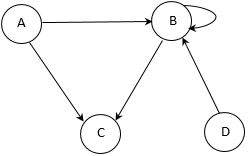
\includegraphics[scale=0.6]{images/Graph1.png}}
	\pause
	$ A =
	\begin{pmatrix}
	0&1&1&0\\
	0&1&1&0\\
	0&0&0&0\\
	0&1&0&0\\
	\end{pmatrix}	
	$
\end{frame}

\begin{frame}{Repräsentation von zweistelligen Relationen durch Matrizen}
	Wir können jede endliche zweistellige Relation durch eine Matrix darstellen!\\
	\textbf{Aufgabe}\\
	Stelle die Kleiner-Gleich-Relation auf der Menge $\{0, 1, 2, 3\}$ dar!\\
	\pause
	$ R_{\leq} =
	\begin{pmatrix}
	1&1&1&1\\
	0&1&1&1\\
	0&0&1&1\\
	0&0&0&1\\
	\end{pmatrix}	
	$
\end{frame}

\section{Erreichbarkeit}
\begin{frame}{Wege-Problem}
	\begin{itemize}
		\pitem Algorithmisches Problem
		\pitem Intuitiv: Gibt es einen Weg von $i$ nach $j$?
	\end{itemize}

	\pause
	
	\begin{block}{Wege-Problem}
		Gegeben einem Graphen $G = (V,E)$. Ist für $i,j \in V$ auch $(i,j) \in E^*$?
	\end{block}

	\pause

	\textbf{Ziel}\\
	\begin{itemize}
		\pitem Gegeben: Adjazenzmatrix
		\pitem Gesucht: Zugehörige \textbf{Wegematrix}, für die gilt:
	\end{itemize}

	\pause

	$W_{ij} = \begin{cases} 
	1 & \text{, falls ein Weg von i nach j existiert}\\
	0 & \text{, sonst}
	\end{cases}$
\end{frame}

\begin{frame}{Einschub Matrizen}
	Was wisst ihr zu folgenden Begriffen?
	
	\begin{itemize}
		\pitem Matrizenmultiplikation
		\pitem Matrizenaddition
		\pitem Potenzieren
		\pitem Einheitsmatrix
		\pitem Nullmatrix
	\end{itemize}
\end{frame}

\begin{frame}{Quadrierte Adjazenzmatrix}
	\textbf{Aufgabe}\\
	Quadriere die Adjazenzmatrix von vorhin:
	$ A =
	\begin{pmatrix}
	0&1&1&0\\
	0&1&1&0\\
	0&0&0&0\\
	0&1&0&0\\
	\end{pmatrix}	
	$
	\pause 
	
	\textbf{Ergebnis}\\
	$ A^2 =
	\begin{pmatrix}
	0&1&1&0\\
	0&1&1&0\\
	0&0&0&0\\
	0&1&1&0\\
	\end{pmatrix}	
	$
\end{frame}

\begin{frame}
	\textbf{Aufgabe}\\
	Bilde und quadriere die Adjazenzmatrix des veränderten Graphen:\\
	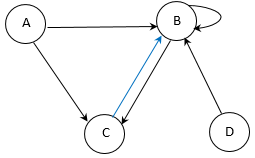
\includegraphics[scale=0.6]{images/Graph2_edit.png}\\
	\pause
	$ A' =
	\begin{pmatrix}
	0&1&1&0\\
	0&1&1&0\\
	0&1&0&0\\
	0&1&0&0\\
	\end{pmatrix}	
	$ 
	und 
	$ A'^2 =
	\begin{pmatrix}
	0&2&1&0\\
	0&2&1&0\\
	0&1&1&0\\
	0&1&1&0\\
	\end{pmatrix}	
	$
\end{frame}

\begin{frame}
	\textbf{Aufgabe}\\
	Was fällt euch auf? Wann steht in $A'^2$ eine $1$, wann eine $2$ und was bedeutet das für unseren Graphen?\\
	$ A' =
	\begin{pmatrix}
	0&1&1&0\\
	0&1&1&0\\
	0&1&0&0\\
	0&1&0&0\\
	\end{pmatrix}	
	$ 
	$ A'^2 =
	\begin{pmatrix}
	0&2&1&0\\
	0&2&1&0\\
	0&1&1&0\\
	0&1&1&0\\
	\end{pmatrix}	
	$ 
	\pause
	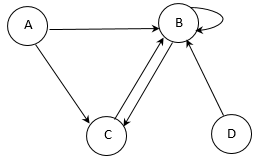
\includegraphics[scale=0.6]{images/Graph2.png} \hspace{0.3cm}\pause
	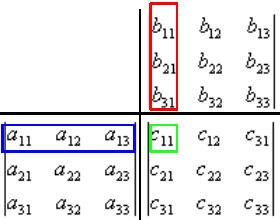
\includegraphics[scale=0.5]{images/multiplikation.png}\\
	\textbf{Tipp:} $c_{11} = a_{11} \cdot b_{11} + a_{12} \cdot b_{21} + a_{13} \cdot b_{31}$
\end{frame}

\begin{frame}
	\textbf{Lösung}\\
	In der $i$-ten Zeile und $j$-ten Spalte von $A^2$ steht die Anzahl der Wege von $i$ nach $j$ der Länge zwei.\\
	\begin{itemize}
		\item[$\rightarrow$]$(A^2)_{ij}$ = Anzahl der Pfade von $i$ nach $j$ der Länge zwei.
	\end{itemize}

	\pause

	\textbf{Aufgabe}\\
	Habt ihr Ideen, wie man herausfindet, zwischen welchen Knoten Pfade der Länge $n$ existieren?\\
	\pause
	\textbf{Lösung}\\
	Betrachte $A^n$!
\end{frame}

\subsection{Zwei-Erreichbarkeit}
\begin{frame}{Zwei-Erreichbarkeit}
	Eigentlich interessiert uns nur, ob ein Pfad der Länge zwei existiert und nicht wie viele...
	\pause
	\begin{block}{Definition Signum-Funktion}
		$sgn: \mathbb{R}\rightarrow \mathbb{R}$\\
		$x \mapsto \begin{cases}
		1& \text{, falls } x > 0\\
		0 & \text{, falls } x = 0\\
		-1& \text{, falls } x < 0
		\end{cases}$
	\end{block}
	\pause
	$sgn(A^2)$ liefert uns die Zwei-Erreichbarkeitsmatrix
\end{frame}

\subsection{Erreichbarkeit}
\begin{frame}
	\textbf{Aufgabe}\\
	Gebe $A^0$, $A^2$ und die Wegematrix $W$ an!
	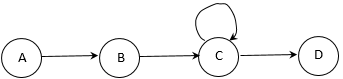
\includegraphics[scale=0.6]{images/Graph3.png}\\
	\pause
	$ A^0 =
	\begin{pmatrix}
	1&0&0&0\\
	0&1&0&0\\
	0&0&1&0\\
	0&0&0&1\\
	\end{pmatrix}	
	$ \pause
	$ A^2 =
	\begin{pmatrix}
	0&0&1&0\\
	0&0&1&1\\
	0&0&1&1\\
	0&0&0&0\\
	\end{pmatrix}	
	$ \pause
	$ W =
	\begin{pmatrix}
	1&1&1&1\\
	0&1&1&1\\
	0&0&1&1\\
	0&0&0&1\\
	\end{pmatrix}	
	$ 
	
\end{frame}

\begin{frame}{Erreichbarkeit}
	Für Pfade beliebiger Länge erhalten wir:
	$W = sgn(A^0 + A^1 + A^2 + A^3 + ...) = sgn(\sum\limits_{i=0}^{\infty} A^i)$\\
	\pause
	Wir können nicht unendlich lange addieren... Ist das ein \textbf{Problem}? 
\end{frame}

\begin{frame}{Erreichbarkeit- unendlich addieren?}
	\ip Wenn ein Pfad $p$ der Länge $ \geq n := |V|$ zwischen $i \neq j$ existiert, muss mindestens ein Knoten doppelt vorgekommen sein! \ip Der Pfad $p$ enthält also einen Zyklus, den wir raus kürzen können.\\\p
	\vspace{0.15cm}
	\textbf{Ergebnis}\\
	Wenn ein Pfad $p$ der Länge $\geq n := |V|$ zwischen $i \neq j$ existiert, existiert auch ein Pfad $p'$ der Länge $< n$.\\\p
	\vspace{0.4cm}
	Für Pfade beliebiger Länge erhalten wir:
	$W = sgn(A^0 + A^1 + A^2 + A^3 + ...) = sgn(\sum\limits_{i=0}^{\infty} A^i)$ \markBlue{$= sgn (\sum\limits_{i=0}^{n-1} A^i)$} \\
\end{frame}

\subsection{Algorithmus}
\begin{frame}{Einfacher Algorithmus zu Berechnung der Wegematrix}
	\only<1>{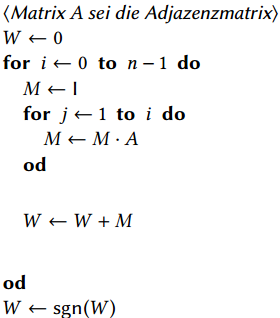
\includegraphics[scale=0.7]{images/algo1.png}}
	\only<2,3>{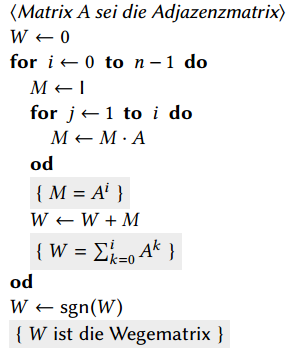
\includegraphics[scale=0.7]{images/algo1_bed.png} 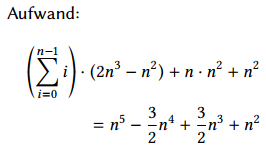
\includegraphics[scale=0.8]{images/aufwand.png} }
	\only<3>{\\ Wie könnte man diesen Algorithmus schneller machen?}
	\only<4>{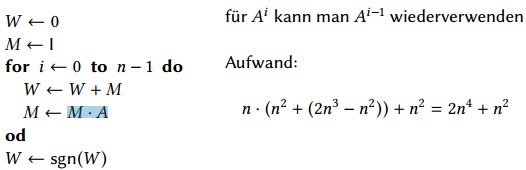
\includegraphics[scale=0.8]{images/algo2.png}}
\end{frame}
\section{Komplexitätstheorie}

\begin{frame}{Komplexitätstheorie}
	\pause
	Wichtige Komplexitätsmaße:
	\begin{itemize}
		\pitem Speicherplatzbedarf
		\pitem Rechen- bzw. Laufzeit
	\end{itemize}
	Unterscheidung in
	\begin{itemize}
		\pitem Best Case (oft uninteressant)
		\pitem Average Case (schwierig zu finden, deswegen selten angegeben)
		\pitem Worst Case  (meistens angegeben)
	\end{itemize}
\end{frame} 

\subsection{O-Notation}
\begin{frame}{Ignorieren konstanter Faktoren}
	\begin{block}{Definition}
		Seien $g,f: \mathbb{N}_0 \rightarrow \mathbb{R}_0^+$ Funktionen. Dann wächst $g$ asymptotisch genauso schnell wie $f$ genau dann, wenn gilt:\\
		$\exists c, c' \in \mathbb{R}_+ : \exists n_0 \in \mathbb{N}_0: \forall n \geq n_0 : c \cdot f(n) \leq g(n)\leq c' \cdot f(n)$
	\end{block}
	\pause

	\textbf{Notation}\\
	$f \asymp g$ oder $f(n) \asymp g(n)$ ("asymptotisch gleich")\\
	\textbf{Bemerkung}\\
	$\asymp$ ist eine Äquivalenzrelation
\end{frame}

\begin{frame}{Theta}
	\begin{block}{Definition}
		$\Theta (f) = \{g|g \asymp f\}$
	\end{block}

	\pause
	
	\begin{block}{Satz}
		$\forall a, b \in \mathbb{R}_+ : \Theta (a\cdot f) = \Theta (b \cdot f)$
	\end{block}
\end{frame}

\begin{frame}{Obere und untere Schranke}
	\begin{block}{Obere Schranke (Worst-Case Approximation)}
		$O(f) = \{g| \exists c \in \mathbb{R}_+ : \exists n_0 \in \mathbb{N}_0: \forall n \geq n_0 : g(n)\leq c \cdot f(n)\}$
	\end{block}

	\pause
	
	\begin{block}{Untere Schranke (Best-Case Approximation)}
		$\Omega(f) = \{g| \exists c \in \mathbb{R}_+ : \exists n_0 \in \mathbb{N}_0: \forall n \geq n_0 : g(n)\geq c \cdot f(n)\}$
	\end{block}
	\pause
	\textbf{Notation}\\
	\begin{itemize}
		\item $g\curlyeqprec f$ falls $g \in O(f)$ bzw. g wächst asymptotisch höchstens so schnell wie f
		\item $g \curlyeqsucc f $ falls $g \in \Omega (f)$ bzw. g wächst asymptotisch mindestens so schnell wie f
	\end{itemize}
	\pause
	\textbf{Bemerkung}\\
	Es gilt $\Theta (f) = O(f) \cap \Omega (f)$
\end{frame}

\begin{frame}
	\begin{block}{Lemma}
		$log_a n \in \Theta (log_b n)$
	\end{block}
	\textbf{Beispiel}\\
	$log_2 n \in \Theta(log_8 n)$\\
	\pause
	\textbf{Beweis}\\
	$\frac{1}{3} log_2 n \ip= \frac{1}{log_2 8} log_2 n \ip= \frac{log_2 n}{log_2 8} \ip= log_8 n \leq log_2 n$
\end{frame}

\begin{frame}
	\textbf{Aufgabe}\\
	Gilt $log_2(n^{20}) \in \Theta (log \space n)$\\
	\pause
	\textbf{Lösung}\\
	Ja, denn $log_2 (n^{20}) = 20 \cdot log_2 n$
\end{frame}

\begin{frame}
	Probeklausur
\end{frame}

\ifdefined\compileall
\else


\ifthenelse{\equal{\compiletype}{print}}
{

\begin{frame}{Informationen}
	
	\begin{columns}
		\begin{column}{0.5\textwidth}
			
			\begin{block}{Zum Tutorium}
				\begin{itemize}
					\item Lukas Bach
					\item Tutorienfolien auf: 
					\begin{itemize}
						\item \url{http://gbi.lukasbach.com}
					\end{itemize}
					\item Tutorium findet statt:
					\begin{itemize}
						\item Donnerstags, 14:00 - 15:30
						\item 50.34 Informatikbau, -107
					\end{itemize}
				\end{itemize}
			\end{block}
			
			\begin{block}{Mehr Material}
				\begin{itemize}
					\item Ehemalige GBI Webseite:
					\begin{itemize}
						\item \url{http://gbi.ira.uka.de}
						\item Altklausuren!
					\end{itemize}
				\end{itemize}
			\end{block}
			
		\end{column}
		\begin{column}{0.5\textwidth}
			
			\begin{block}{Zur Veranstaltung}
				\begin{itemize}
					\item Grundbegriffe der Informatik
					\item Klausurtermin:
					\begin{itemize}
						\item 06.03.2017, 11:00
						\item Zwei Stunden Bearbeitungszeit
						\item 6 ECTS für Informatiker und Informationswirte, 4 ECTS für Mathematiker und Physiker
					\end{itemize}
				\end{itemize}
			\end{block}
			
			\begin{block}{Zum Übungsschein}
				\begin{itemize}
					\item Übungsblatt jede Woche
					\item Ab 50\% insgesamt hat man den Übungsschein
					\item Keine Voraussetzung für die Klausur, aber für das Modul
				\end{itemize}
			\end{block}
			
		\end{column}
	\end{columns}
	
\end{frame}

}{}

\ifdefined\livebeamermode
	\begin{frame}
		
\includegraphics[width=\linewidth]{images/thatsall.png}
	\end{frame}
\fi

\end{document}

\fi